\ifx\wholebook\relax\else
\input{../Common.tex}
\input{../macroes}
\begin{document}
\fi

\chapter{Looping}\label{ch:looping}\label{cha:loops}

\begin{chapterfigure}
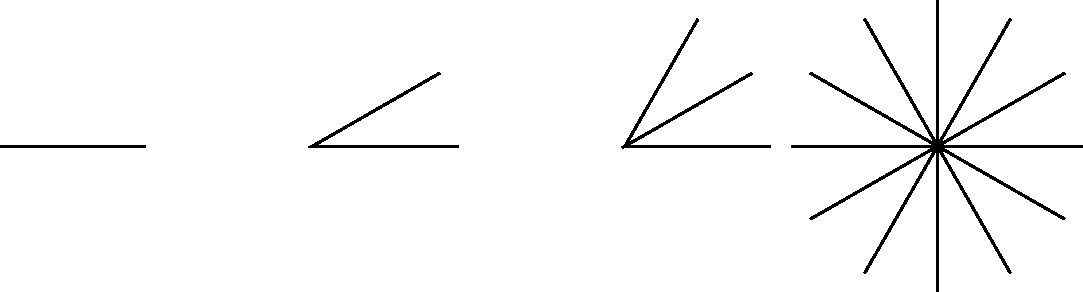
\includegraphics[width=0.9\linewidth]{loopTitlePicture}
\end{chapterfigure}

\hidden{
|caro|
caro := Turtle new.
caro west; jump: 300;east.
caro  go: 70.
caro  turnLeft: 180.
caro go: 70.
caro turnLeft: 180.

caro jump: 150.
2 timesRepeat: [ caro  go: 70.
				caro  turnLeft: 180.
				caro go: 70.
				caro turnLeft: 180.
				caro turnLeft: 30].
caro east.
caro jump: 150.
3 timesRepeat: [ caro  go: 70.
				caro  turnLeft: 180.
				caro go: 70.
				caro turnLeft: 180.
				caro turnLeft: 30].
caro east.
caro jump: 150.
12 timesRepeat: [ caro  go: 70.
				caro  turnLeft: 180.
				caro go: 70.
				caro turnLeft: 180.
				caro turnLeft: 30]
}


By now you must think that the job of turtle tamer is quite
tedious. We are sure that you have ideas of nice drawings, but you did not get the hart to draw scripts to draw them.  Indeed, the amount of things to type gets larger and larger as the complexity of the drawing augments. In this chapter, you will learn how to reduce the amount of commands given to a turtle using loops. Loops allow one to \emph{repeat a sequence of messages}. With a loop, the script drawing a square is no bigger than the one drawing an hexagon or an octagon.

\section{A Star}
We would like that a turtle draws a star as shown in the picture above. The principle is the following one: A turtle has to draw a line, comes back to its previous location, turns from a certain angle and draws another line and so on. The \scriptref{scr:line} makes a turtle drawing a line of 70 pixels
and coming back to its previous location. Note that in addition, after having drawn the line the turtle points in the same direction where it was pointing before drawing the line.

\begin{scriptwithtitle}{Drawing a line and coming back}\label{scr:line}
| caro |
caro := Turtle new.
caro go: 70.
caro turnLeft: 180.
caro go: 70.
caro turnLeft: 180.
\end{scriptwithtitle}

Now to draw a star, we have to \emph{repeat} the \scriptref{scr:line} and make the turtle turns from a given angle, for example 60
degree. The \scriptref{scr:star} shows how this should be done to
obtain a star having 6 branches without using loops.

\begin{scriptwithtitle}{A star without loop!}\label{scr:star}
| caro |
caro := Turtle new.
caro go: 70.
caro turnLeft: 180.
caro go: 70.
caro turnLeft: 180.
caro turnLeft: 60. 
\textit{caro go: 70.
caro turnLeft: 180.
caro go: 70.
caro turnLeft: 180.
caro turnLeft: 60.}
caro go: 70.
caro turnLeft: 180.
caro go: 70.
caro turnLeft: 180.
\textit{caro turnLeft: 60. 
caro go: 70.
caro turnLeft: 180.
caro go: 70.
caro turnLeft: 180.
caro turnLeft: 60.} 
caro go: 70.
caro turnLeft: 180.
caro go: 70.
caro turnLeft: 180.
caro turnLeft: 60. 
\textit{caro go: 70.
caro turnLeft: 180.
caro go: 70.
caro turnLeft: 180.
caro turnLeft: 60.} 
\end{scriptwithtitle}

As you see, this is clearly boring to have to type all this code that
does all the time the same thing. Imagine if we would like to have a
star with 60 branches like the star shown in the
\scriptref{scr:starsixty}! In fact we would like to be able to 
repeat a sequence of messages.

\paragraph{Using a  Loop.} There is a solution to this problem: using a \emph{loop!} There are different kinds of loops like iterating while a certain condition holds or a given  number of times. For the moment the loop we present allows one to repeat a given sequence of messages a given number of times. The method \timesRepeat  \index{timesRepeat:} allows one to define a loop  that will repeat a sequence of  messages a given number of times like shown in the \scriptref{scr:starloop}. The \scriptref{scr:starloop} defines the same star than the 
\scriptref{scr:star} but in a much smaller way. 

\begin{scriptwithtitle}{A star with a loop}\label{scr:starloop}
| caro |
caro := Turtle new.
6 timesRepeat: 
     \textbf{\textbf{[}caro go: 70.
     caro turnLeft: 180.
     caro go: 70.
     caro turnLeft: 180.
     caro turnLeft: 60\textbf{]}}
\end{scriptwithtitle} 

\important{\ct{n timesRepeat: [ ...foo...]} repeat n times \ct{...foo...}}


The method \timesRepeat allows one to repeat a sequence of messages a given number of times. In \sq such a sequence of messages delimited by \ct{[} and \ct{]} is called a \emph{block}. Another interesting point is that \timesRepeat is not sent to a turtle but to an integer, the number of times the sequence should be repeated. In the
\scriptref{scr:starsixty} the message \timesRepeat: \ct{[...]} is sent
to \ct{60}. Finally note that the number receiving the message \timesRepeat have to be an \emph{integer} because as in real life there is no sense to do a sequence of 
messages 0.2785 times for example.

\ 
\begin{template}
\textit{n} \textbf{timesRepeat:}
   \textbf{[} \textit{sequence of messages} \textbf{]}
\end{template}
\ 


Type the \scriptref{scr:starloop} and change the number of
times the loop is repeated by replacing \ct{6} by the number you want.
Pay attention that \ct{60} should be changed accordingly if you want
to generate a complete star. To have a complete star the relation
between the angle and the number of repetition should be $angle * n =
360$. In the \scriptref{scr:starsixty} the loop is repeated 60 times and the angle is 6 degree, so the star is complete. 

\begin{scriptfig}{loopStar60}{A star with 60 branches}\label{scr:starsixty}
| caro |
caro := Turtle new.
60 timesRepeat: 
      \textbf{[}caro  go: 70.
      caro  turnLeft: 180.
      caro go: 70.
      caro turnLeft: 180.
      caro turnLeft: 6\textbf{]}
\end{scriptfig}


\begin{teacher} \textbf{About code indentation}\\
In \st, the code can be layouted in all kind of ways and the indentation (its shape regardings the left margin) has no semantics. However, using a clear indentation really helps the reader to understand the code. We suggest to follow the convention we chose to format \ct{timesRepeat:} expressions. The idea is that the repeated block of expressions delimited by the characters \ct{[} and \ct{]} should form a visual and textual rectangle. That is why we start the block with \ct{[} on the next line after the \ct{timesRepeat:} and align all the expressions inside the block to one tab and finish by \ct{]} that indicates that the block ends. Note that code formatting is one of the most complex topics because different people like to read their code in different ways and because often esthetism does not like regularity. So the one we propose is primarily focused at helping the identification of the repeated messages as illustrated in the following code

\begin{alltt}
60 timesRepeat: 
      [caro  go: 70.
      caro  turnLeft: 180.
      caro go: 70]
\end{alltt}
\ 
\end{teacher}

\section{Typing in the Air}
If you want to type directly the code of your loops using the balloon, you should realize that you need a way to tell that certain messages are sent to the turtle itself, this is exactly the purpose of the word \ct{self} in \sq. 
Figure~\ref{fig:fourtimesRepeat} shows how we can directly ask a turtle to draw a square with and without cascade. We will also see that \ct{self} is really necessary when we will define new kind of messages in Chapter~\ref{ch:abstraction}.

\begin{figure}[!h]\centerline{\includegraphics{balloonSelf4timesRepeat}}\centerline{\includegraphics{balloonSelf4timesRepeatCascade}}
\caption{Using \ct{self} to refer to the turtle that will receive the messages \ct{go: 100} and \ct{turnLeft: 90}. \label{fig:fourtimesRepeat}}\end{figure}



\section{Exercising Regular Shapes}
As you may have noticed, some figures can be obtained by simply
repeating sequences of messages, especially the ones produced in
Section~\ref{sec:firstPolygons} of Chapter~\ref{ch:relativeTurn} (repeated here as the script~\ref{scr:boucl:relativeSquare}). 

%\begin{scriptfigwithsize}[0.4]{
\includegraphics[width=4cm]{loopFirstSquare}}{A first square} \label{scr:boucl:relativeSquare}
%| caro |
%caro := Turtle new.
%caro go: 100.
%caro turnLeft: 90.
%caro go: 100.
%caro turnLeft: 90.
%caro go: 100.
%caro turnLeft: 90.
%caro go: 100.
%caro turnLeft: 90
%\end{scriptfigwithsize}

\begin{scriptwithtitle}{A first square} \label{scr:boucl:relativeSquare}
| caro |
caro := Turtle new.
caro go: 100.
caro turnLeft: 90.
caro go: 100.
caro turnLeft: 90.
caro go: 100.
caro turnLeft: 90.
caro go: 100.
caro turnLeft: 90
\end{scriptwithtitle}


\begin{exonofig}\label{exo:squareRepeat}
Granted, that the last \turnLeft message is not really needed, but it
does no harm, transform the \scriptref{scr:boucl:relativeSquare} to
draw the same square but using the command \timesRepeat.
\end{exonofig}

Now you should be able to draw other regular polygons with a large
number of sides.


\begin{exofigwithsize}{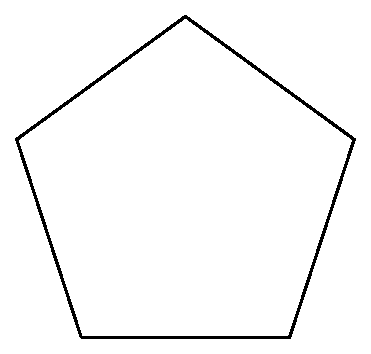
\includegraphics[width=4cm]{loopPentagon}} \label{exo:pentagonRepeat}
Draw a pentagon using the method \timesRepeat.
\end{exofigwithsize}

\begin{exofigwithsize}{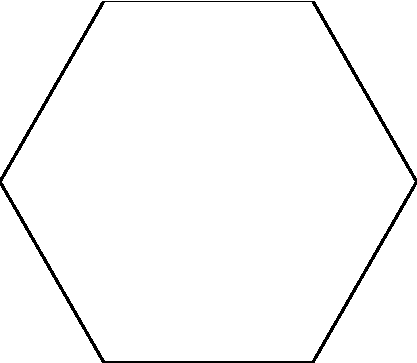
\includegraphics[width=4cm]{loopHexagon}}\label{exo:hexagonRepeat}
Draw a hexagon using the command \timesRepeat.
\end{exofigwithsize}


If you get the hang of it, try to augment the number of sides of a
polygon to a very large number. You may need to reduce the size of
the sides so that figure fits within the screen. When the
number of sides is large and the size of the sides is small, the
polygon will look like a circle.


\section{Pyramids Rediscovered}\label{sec:bouclonpyramids}
Remember how you coded the outline of the pyramid of Saqqarah in
\exoref{exo:saqqarah}? You can simplify your drawing by using a loop 
as follows:

\begin{scriptfig}{loopPyramid}{Pyramid script} \label{scr:pyramid}
| caro |
caro := Turtle new.
5 timesRepeat: 
     [caro north.
     caro go: 20.
     caro east.
     caro go: 20].
5 timesRepeat: 
     [caro go: 20.
     caro south.
     caro go: 20.
     caro east].
caro west.
caro go: 200.
\end{scriptfig}

Now should should be able to generate pyramids with any number of
terraces \emph{with the same number of commands}, just by changing
the numbers of the script.

\begin{exofig}{loopPyramid10} \label{exo:pyramid}
Try to draw a pyramid with 10 terraces using a variation of Script~\ref{scr:pyramid}.
\end{exofig}

You may want to generate pyramids with an even larger number of
terraces. The size of the terraces must be adjusted if you want
them to fit within the screen.

\section{Problems to solve}
As you have seen, the generation of the pyramid involves the
repetition of a block of code, which draws two line elements. Once the
proper repeating element is identified, one can produce complex
picture from elementary drawing, by repeating themselves.  The
following exercises illustrate this principle.

\begin{exofigwithsizeandtitle}{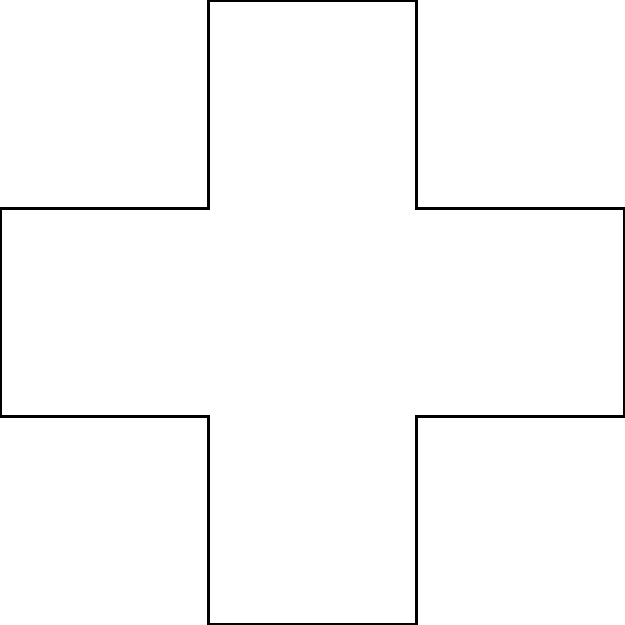
\includegraphics[width=4cm]{loopCross}}{Red Cross} \label{exo:redcross}
Draw the outline of the Red Cross using \turnLeft or \turnRight and
\timesRepeat.
\end{exofigwithsizeandtitle}


\begin{exofigwithtitle}{loopStair}{Stair}\label{exo:stair}
Draw the following stair.
\end{exofigwithtitle}


\hidden{| caro |
caro := Turtle new.
10 timesRepeat: [ caro go: 10.
                caro north.
                caro go: 10.
                caro east]}

\begin{exofigwithtitle}{loopStylisedStair}{Stylized Stair}\label{exo:stylizedstair}
Draw the following stylized stair.
\end{exofigwithtitle}
\hidden{loopstylisedstair

	| caro |
	caro := Turtle new.
	10 timesRepeat: [
                caro go: 10.
                caro north.
                caro jump: 10.
                caro east]}

\begin{exofigwithsizeandtitle}{
\includegraphics{loopSimpleElement}}{A Simple Element}\label{exo:element}
Draw the following graphical element.
\end{exofigwithsizeandtitle}


\hidden{
| caro |
caro := Turtle new.
caro north. 
caro go: 25.
caro west.
caro go: 25.
caro south.
caro go: 25}


\begin{exofigwithsizeandtitle}[0.3]{
\includegraphics{loopComb}}{Comb}\label{exo:comb}
Transform the \scriptref{exo:element} to produce a comb.
\end{exofigwithsizeandtitle}

\hidden{
| caro |
caro := Turtle new.
8 timesRepeat: [caro north. 
caro go: 25.
caro west.
caro go: 25.
caro south.
caro go: 25]}


\begin{exofigwithsizeandtitle}{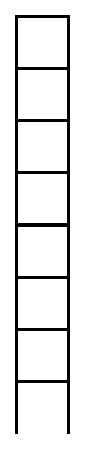
\includegraphics{loopLadder}}{Ladder}\label{exo:ladder}
Transform the \scriptref{exo:element} to produce a ladder.
\end{exofigwithsizeandtitle}


\hidden{
| caro |
caro := Turtle new.
8 timesRepeat: [caro north. 
caro go: 25.
caro west.
caro go: 25.
caro south.
caro go: 25.
caro north.
caro jump: 25.
caro east.
caro jump: 25]}


\begin{exonofig}
Now that you master loops define a loop that draws the tumbling squares of the picture shown at the opening of chapter~\ref{ch:relativeTurn}.
\end{exonofig}


\section{Some Remarks about Loops}
Up until now we presented loops that repeated a number of times
a sequence of messages and this number of repetition was always known when we were defining the script. However, this does not have to be the case and the number of iteration can be just a number returned as a result of a calculation or even interaction with the user. This is what we will illustrate now.
Let us take a simple example, imagine that we want to let the user chose the number of step a stair should have. The script~\ref{scr:interactive} illustrates one possibility to ask the user some input values. A possible execution is shown in Figure~\ref{fig:usertroismarches}.


%\begin{teacher}We said that loops allows one to avoid the duplication of similar instructions. This is true but we could imagine powerful programming environments that would help us to manage repetitions without having to have explicit support for loops at the level of the language. The text editor could copy the code we want to repeat the number of time we want and we would not need explicit loop methods such as \timesRepeat. This hypothesis could hold but there are cases where we do not know the number of times we want to loop {\em when we are writing the code}. In reality most of loops are defined to iterate a number of times that is not defined at the moment the loop is written but at execution or depending of other parameters. \end{teacher}


\begin{figure}[!htbp]
\begin{minipage}[b]{.5\linewidth}
\centerline{\includegraphics{nbMarches}}
\end{minipage}
\begin{minipage}[b]{.5\linewidth}
\centerline{\includegraphics{threeStair}}
\end{minipage}
\caption{The system asks the number of stairs that the user would like with 10 as default value. The user enters 3.}
\label{fig:usertroismarches}
\end{figure}


\begin{scriptfig}{interactiveStair}{Interactive stair}\label{scr:interactive}
| caro number | 
number := (FillInTheBlank 
            request: 'Number of steps' 
            initialAnswer: '10') \textbf{asNumber}. 
caro := Turtle new.
number timesRepeat:  
   [caro go: 10.
   caro north.
   caro go: 10.
   caro east]
\end{scriptfig}


The expression  \ct{FillInTheBlank request: 'Number of steps'  initialAnswer: '10')} \index{FillInTheBlank} creates a small
widget that asks some input from the user as shown in figures~\ref{fig:usertroismarches}. Exactly the message
\ct{request: aString initialAnswer: anotherString} is sent to \ct{FillInTheBlank}\footnote{\ct{FillInTheBlank} is a class, \ie a factory of this kind of small widgets.} It requires to specify a text that explains to the user the requested value, and a default value to help him. If the user does not change the default value, it will be returned. The text and the default value are specified as \textit{strings}. A string is a collection of characters. It is delimited by single quotes \ct{'}. \ct{'Number of steps'}  is a string. 

The created widget is then waiting for the user to optionally specify a value and to press the buttons accept or cancel. 
It returns also a string representing the value specified by the user. The script expects that the user enters a number. Note that there is no verification of possible wrong edition. Experiment a bit by evaluating the following code and printing its returned value (print it). 

\begin{alltt}
(FillInTheBlank request: 'Combien de marche' initialAnswer: '10')
\end{alltt}

Note that the returned value is a string and not a number. However, the method \ct{timesRepeat:} has to be sent to an integer, so we have to transform the string, the textual representation of a number into the number itself. This could be a tedious task but we can use the method \ct{asNumber}\index{asNumber} that when sent to a string representing a number returned this number. 


\begin{sqref}
A string \index{String} is a collection of characters \index{character} delimited by single quotes. For example, 
the following expressions are also strings: 
\begin{description}
\item{}\ct{'a'} is a string composed by only one character. 
\item{\ct{'smalltalk'}} is a string  composed by several characters.
\item{\ct{'number of steps de marches'}} is a string  composed by several characters including spaces. 
\item{\ct{'Don't do that'}} if you want to include a single quote inside a string you simply double it. 
\item{\ct{'10'}} is a string composed by two characters: the character \ct{1} and the character  \ct{0}.
\item{\ct{'small','talk'} returns a new string \ct{'smalltalk'}}. To concatenate\index{concatenation} two strings, we send the message \ct{,}\index{,} to the first one with the second as argument. 
\end{description}

A character is also an object and it starts by a dollar sign \texttt{\$}.
For example,  the following expressions are characters: 
\begin{description}
\item{\texttt{\$a}, \texttt{\$O}, \texttt{\$?}, \texttt{\$\^}} are characters.
\item Invisible characters are created by sending message to the class \ct{Character}. For example \ct{Character space} returns the character representing a space. 
\item \texttt{\$A asString} returns \ct{'A'} a string containing the character  \texttt{\$A}
\end{description}
\end{sqref}

\subsection*{Using Random Numbers}
Another example showing that the number of times a loop should be executed is not always known when the loops is defined is  to pick a number at random and execute the loop this number of times. To get a random number between 1 and a given number, we send to this number the message \index{atRandom}\ct{atRandom} as shown by \tscrref{scr:nbaleatoire}. 

\begin{scriptwithtitle}{ObtainingRandom number between 1 and 100}\label{scr:nbaleatoire}
100 atRandom
\end{scriptwithtitle}

\begin{teacher}
In \st everything is an object that understands messages, hence numbers are also objects. Here \ct{100} is an object and \ct{atRandom} is a method defined on numbers.  
\end{teacher}

\begin{scriptwithtitle}{Random stair}\label{scr:random}
| caro number | 
number := 10 atRandom. 
caro := Turtle new.
number timesRepeat: 
       [caro go: 30.
       caro north.
       caro go: 30.
       caro east]
\end{scriptwithtitle}

\begin{teacher}
If you want to check the numbers generated, open a transcript as explained in chapter~\charef{cha:Tour} and evaluate \tscrref{scr:nbaleatoires}. The transcript is always present in the system that is used to display system information and program traces. It is handy and a cheap way to follow the behavior of programs.
The \ct{Transcript} understands  message \ct{show:} \index{show:} and \ct{cr}. \ct{show:} \index{show:} asks the transcript  to display a string and \ct{cr} indicates to the transcript to introduce a new line (a carriage return - hence cr)  in its text field. \tscrref{scr:nbaleatoires} defines a loop that generates a randow number between 1 and 100 and transformed it into a string by sending to the   generated number the message \ct{printString} and finally asks the Transcript to display it (see Figure~\ref{fig:usertroismarchesontr}). 
\end{teacher}

\begin{figure}[!htbp]
\centerline{\includegraphics[width=10cm]{numbersOnTranscript}}
\caption{Using a workspace and a transcript to compute and display random numbers.
\label{fig:usertroismarchesontr}}
\end{figure}

\begin{scriptwithtitle}{Displaying 200 random numbers between 1 and 100}\label{scr:nbaleatoires}
200 timesRepeat: 
   [Transcript  show: 100 atRandom printString. 
   Transcript cr]
\end{scriptwithtitle}




\summa

\begin{table}[h]
\centering
\begin{tabular}{||p{3cm}|p{4cm}|p{6.5cm}||} \hline
% after \\ : \hline or \cline{col1-col2} \cline{col3-col4} ...
Method&Description&Example\\[1ex] \hline
\emph{\ct{n}} \timesRepeat \ct{[\emph{xxx}]}&repeats \emph{n} times a sequence of messages
&\begin{alltt}
10 timesRepeat: 
    [caro go: 10. 
    caro jump: 10]\end{alltt} \\ \hline
\ct{aString asNumber}&Returns the number represented by aString& \ct{'123' asNumber} returns the number \ct{123} \\ \hline
\ct{aNumber printString}&Returns the textual representation of a number& \ct{123 printString} returns the string \ct{'123'}. 
\ct{123 printString asNumber} returns the number itself \ct{123}.
\\ \hline
\ct{aNumber atRandom}&Generates a number randomly between 1 and aNumber& \ct{100 atRandom}\\ \hline
\ct{Transcript show: aString}& Diplays aString into the Transcript&\ct{Transcript show: 'hello'}\\ \hline
\ct{Transcript cr}&Add a carriage return into the Transcript&\\ \hline
\end{tabular}
\end{table}



\ifx\wholebook\relax\else\end{document}\fi


